\documentclass{article}
 
% if you need to pass options to natbib, use, e.g.:
%     \PassOptionsToPackage{numbers, compress}{natbib}
% before loading neurips_2019
 
% ready for submission
% \usepackage{neurips_2019}
 
% to compile a preprint version, e.g., for submission to arXiv, add add the
% [preprint] option:
    \usepackage[preprint]{neurips_2019}
 
% to compile a camera-ready version, add the [final] option, e.g.:
    %  \usepackage[final]{neurips_2019}
 
% to avoid loading the natbib package, add option nonatbib:
%     \usepackage[nonatbib]{neurips_2019}
 
\usepackage[utf8]{inputenc} % allow utf-8 input
\usepackage[T1]{fontenc}    % use 8-bit T1 fonts
\usepackage{hyperref}       % hyperlinks
\usepackage{url}            % simple URL typesetting
\usepackage{booktabs}       % professional-quality tables
\usepackage{amsfonts}       % blackboard math symbols
\usepackage{nicefrac}       % compact symbols for 1/2, etc.
\usepackage{microtype}      % microtypography
\usepackage{graphicx}
\title{CSCI5622 Fall 2019 Group Project: MiMic\\
       Project Proposal and Midpoint Report}
 
% The \author macro works with any number of authors. There are two commands
% used to separate the names and addresses of multiple authors: \And and \AND.
%
% Using \And between authors leaves it to LaTeX to determine where to break the
% lines. Using \AND forces a line break at that point. So, if LaTeX puts 3 of 4
% authors names on the first line, and the last on the second line, try using
% \AND instead of \And before the third author name.
 
\author{%
  Nirvan S P Theethira\\
%  Department of Computer Science\\
%  University of Colorado Boulder\\
  \texttt{nith5605@colorado.edu} \\
  \And
  Charlie Carlson\\
%  Department of Computer Science\\
%  University of Colorado Boulder\\
  \texttt{chca0914@colorado.edu} \\
  \And
  Ketan Ramesh\\
  \texttt{kerk1228@colorado.edu} \\
  \And
  Pramod Venkatesh Kulkarni\\
%  Department of Computer Science\\
%  University of Colorado Boulder\\
  \texttt{prku8035@colorado.edu} \\
}
 
\begin{document}
 
\maketitle
 
\begin{abstract}
 After careful consideration we have decided to change projects.
 Our original proposed project was to use the Google Quick Draw! data set to train a neural network to classify small hand-drawn sketches.
 We discovered that not only had many others already attempted this but they had posted their code online and used similar models to those we had hoped to try.
 Thus, to avoid redundancy, we are switching to a different project which we believe to be slightly more novel and much more interesting. 
 Our new project is to train a chatbot with the personality of a TV show character.
 This document will serve both as a new project proposal and midpoint report where we will both review what we plan to do and report what we have already done to meet midpoint expectations.
\end{abstract}
 
\section{Project Proposal}
%\subsection{Motivation}
A chatbot is a program that provides conversational output in response to user input.
They have many applications such as customer support interfaces, general question answering services, translation apps and virtual assistants.
A common goal for chatbots is to simulate a human like interaction for the user.
To this end many researches have investigated creating chatbots which can do more than just factually answer questions \cite{Li2016, LINH2019, QianHZXZ17, ZhouHZZL17,NMC2017}.
That is, they have investigated creating chatbots which have "personality" or "identity."
In this work we propose attempting to train a neural network to act as a chatbot which simulates a known personality.
Namely, we want to train a neural network to react as TV show personalities.
 
%\subsection{Justification}
A Sequence-to-sequence model is a general purpose encoder-decoder model that can take structured text as input and output similarly structured text.
For example, they can take in English sentences and output English sentences.
Such models are regularly used to model translation, summarization and conversational tasks.
We propose using such a model to train our TV personality chatbot as it is similar task.
%\subsection{Dataset}
 
For a data set, we will use transcripts from popular TV shows such as Friends and consider statement response pairs from scene dialogue.
That is, for each scene in an episode we parse out the dialogue in order and pair them sequentially.
Each dialogue instance includes the character speaking and the actual dialogue.
We call the first dialogue instance a statement and the second a response.
\begin{table}
  \caption{Example data point}
  \label{sample-data}
  \centering
  \begin{tabular}{ c | c l }
    Type  & Character & Dialogue \\
    \hline
    Statement:  & Charlie:  & "This project is awesome!"    \\
    Response:   &  Ketan: & "Yes it is!"     \\
    \bottomrule
  \end{tabular}
\end{table}
For each character of interest, we collect all pairs such that the character is the responder. 
We then train our model with the goal of it learning to react to input from any statement maker as the responder.
Focusing on TV characters with strong personalities, we hope that after sufficient training, the chatbot will noticeably behave like the character of interest.
For the interest of both automatic and human based metrics, we will reserve about 30\% of our collected data for each character as test data.
 
While the task and goal for this project are clear, a major question is how to measure performance.
It  is believed that measuring the performance of such chatbots is difficult \cite{Radz2017, Xing2018, LiuLSNCP16,Devlin2018,SerbanLCP15}.
We propose using several metrics to measure our chatbot's final performance.
While they are not usually very good indicators we will consider automatic metrics such as BLEU and METEOR.
We will also look into more modern automatic metrics that have recently been introduced to measure the performance of personality based chatbots \cite{Xing2018}.
Finally, we will construct human evaluation metrics which is fairly standard for chatbot evaluation. 
An example idea is to ask a human to determine if a reported response does represent some notion of the character's personality.
When designing theses human evaluation questions, we will have to careful consider the audience and create questions that will hopefully let us understand both how well our chatbot appears to hold a conversation and how well it matches the desired personality.

 
\section{Midpoint Report}
As of submitting this document we have collected and parsed our first dataset, the transcript for dialogue for the popular TV show Friends.
We hope to collect additional data from other popular TV shows as well for our final result.

\subsection*{F.R.I.E.N.D.S Dataset}
The chatbot training trials were started with the friends data set. The dataset was retrieved from: \url{https://fangj.github.io/friends/}. The text file are split up by episodes. Each text file contains dialogue scrips that indicate the character speaking. The scripts also indicate scene transitions.\\
\begin{figure}[h]
  \centering
  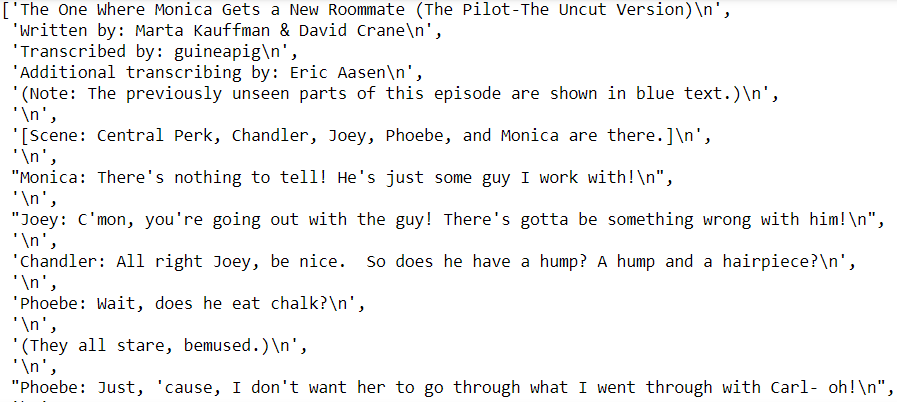
\includegraphics[width=140mm]{rawData.PNG}
  \caption{Raw Data.}
\end{figure}

For the basic implementation, the TV character 'Joey' was used. 
We collected all input-response pairs from every episode where Joey was the responder.
%All dialogues said by Joey were sampled and used for the output and every dialogue said right before Joey's dialogue were sampled and used for the input. 
The input and output were tab separated and saved in a text file. 
This formed 8000 input-response pairs that were used to train a sequence-to-sequence model.
\begin{figure}[h]
  \centering
  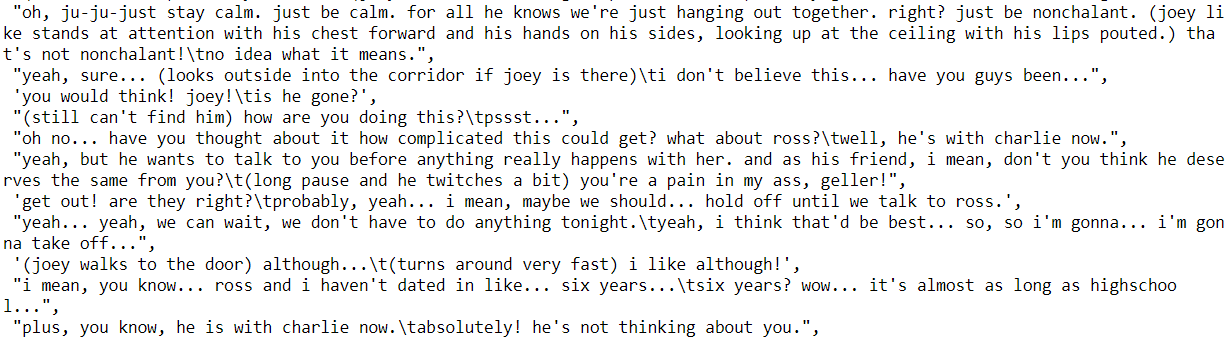
\includegraphics[width=120mm]{processedData.PNG}
  \caption{Joey dialogue traning data.}
\end{figure}

\subsection*{Baseline Model - Seq2Seq}
Sequence-to-Sequence learning deals with training models to convert sequences from one domain to another. Most common uses include Language translation but, the task can be extended to work for free-form question answering or any task involving text generation.
The model takes in an input of variable length and produces a variable length output. The model contains an RNN/ LSTM that acts as an Encoder. The Encoder processes the inputs, encoding the information as internal states. These internal states act as context/conditioning in the decoding steps. The outputs of the Encoder are ignored. The Decoder, made up of an RNN/ LSTM is trained to predict the next character, given the hidden states formed by the Encoder. The output at each time step of the decoding phase is used as the input for the next time step leading to text generation.
\begin{figure}[h]
  \centering
  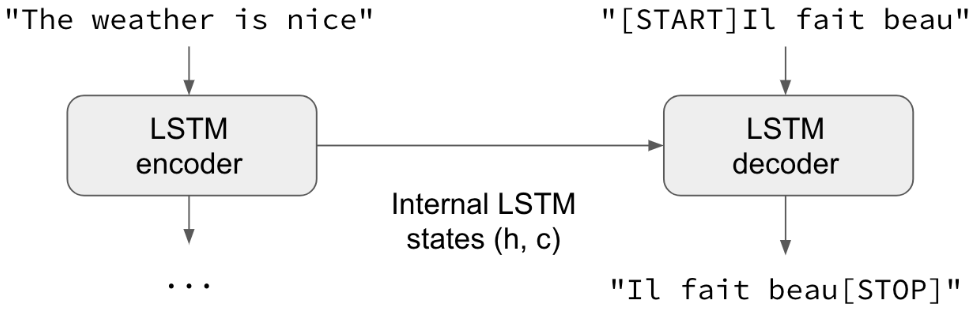
\includegraphics[width=120mm]{seq2seq.PNG}
  \caption{Baseline Seq2Seq Model Structure.}
\end{figure}

The model is trained on the data set described above.
%F.R.I.E.N.D.S dataset containing transcripts of each episode across 10 seasons. 
The Encoder is trained to generate hidden states for dialogues whereas the Decoder is trained to generate responses conditioned on Joey's responses.
\begin{figure}[h]
  \centering
  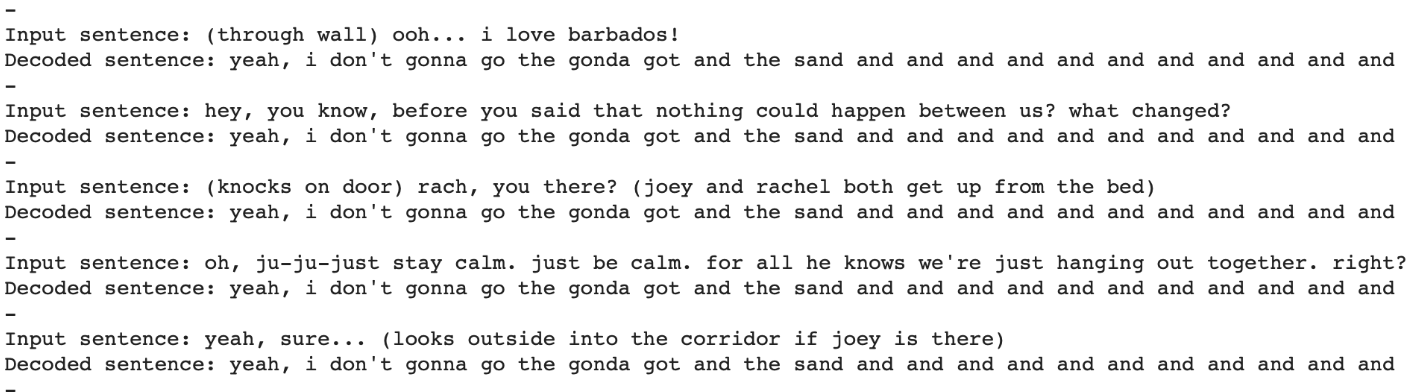
\includegraphics[width=100mm]{initOutput.PNG}
  \caption{Sample output after 10 epochs.}
\end{figure}

\subsection*{Next Steps}
Moving forward we have identified several key tasks that we want to complete in the next few weeks:
\begin{enumerate}
	\item Collect additional data sets from other TV shows such as Big Bang Theory, Lost, Game of Thrones and The Simpsons.
	\item Finalize and implement automatic metrics for evaluating chatbot performance.
	\item Tune a sequence-to-sequence model and run on full data sets to train personality chatbot.
	\item Research and implement strategies for human based evaluation metrics.
\end{enumerate}
We have also considered a few reach goals that we would like to consider moving forward:
\begin{enumerate}
	\item Research and implement other models to train same data set. One example is to use BERT \cite{Devlin2018}.
	\item Create a user interface for interaction with trained personality chatbots.
	\item Consider using a much larger data set for general human text interaction in hopes of increasing quality of trained model's responses.
\end{enumerate}

\bibliography{references}
\bibliographystyle{unsrt}

\end{document}